\section{Experimentación}
La experimentación consistió en capturar el tráfico de paquetes, utilizando la herramienta previamente desarrollada, en las siguientes redes: una red hogareña, un McDonalds, un Starbucks, el laboratorio del DC y en el Subte.

La herramienta desarrollada no solo captura el tráfico de paquetes, sino que también hace una distinción de tipos de paquetes (qué protocolos usan), y en caso de que sean ARP toma su IP destino. Luego, con esta información se procede a calcular las probabilidades de aparición de cada tipo de paquete, contando la cantidad de apariciones de un paquete sobre el total de los paquetes capturados. De manera análoga se calcula las probabilidades de aparición de las IPs destino en los paquetes ARP. Una vez calculadas las probabilidades, es fácil realizar el cálculo de información de cada evento y las entropías de las distintas fuentes, aplicando las fórmulas presentadas en la sección de \textit{Desarrollo}.

Luego se realizaron histogramas para tener una visualización de la cantidad de apariciones de cada evento, asi también como la información de los mismos.
Por último, realizamos un grafo que representa el tráfico de paquetes en cada red, para poder comprender con mayor claridad lo que sucede en ellas.

\newpage

\subsection{Red Hogareña}

En este experimento, capturamos los paquetes de la LAN de uno de los miembros de nuestro grupo. La medición fue realizada un día sábado desde las 12 hs hasta las 14 hs. La cantidad de paquetes capturados aproximadamente es de 125000. Sin embargo, sólo 153 de estos corresponden al protocolo ARP.

\newpage

\subsection{Red McDonald's}

Para el siguiente experimento, capturamos los paquetes de la LAN Wi-Fi pública del McDonald's ubicado en el shopping Alto Avellaneda. La medición fue realizada un día sábado desde las 18 hs hasta las 20 hs. La cantidad de paquetes capturados es de aproximadamente 65.000. De todos estos, sólo 918 corresponden al protocolo ARP.

\begin{figure}[H]
       \centering
       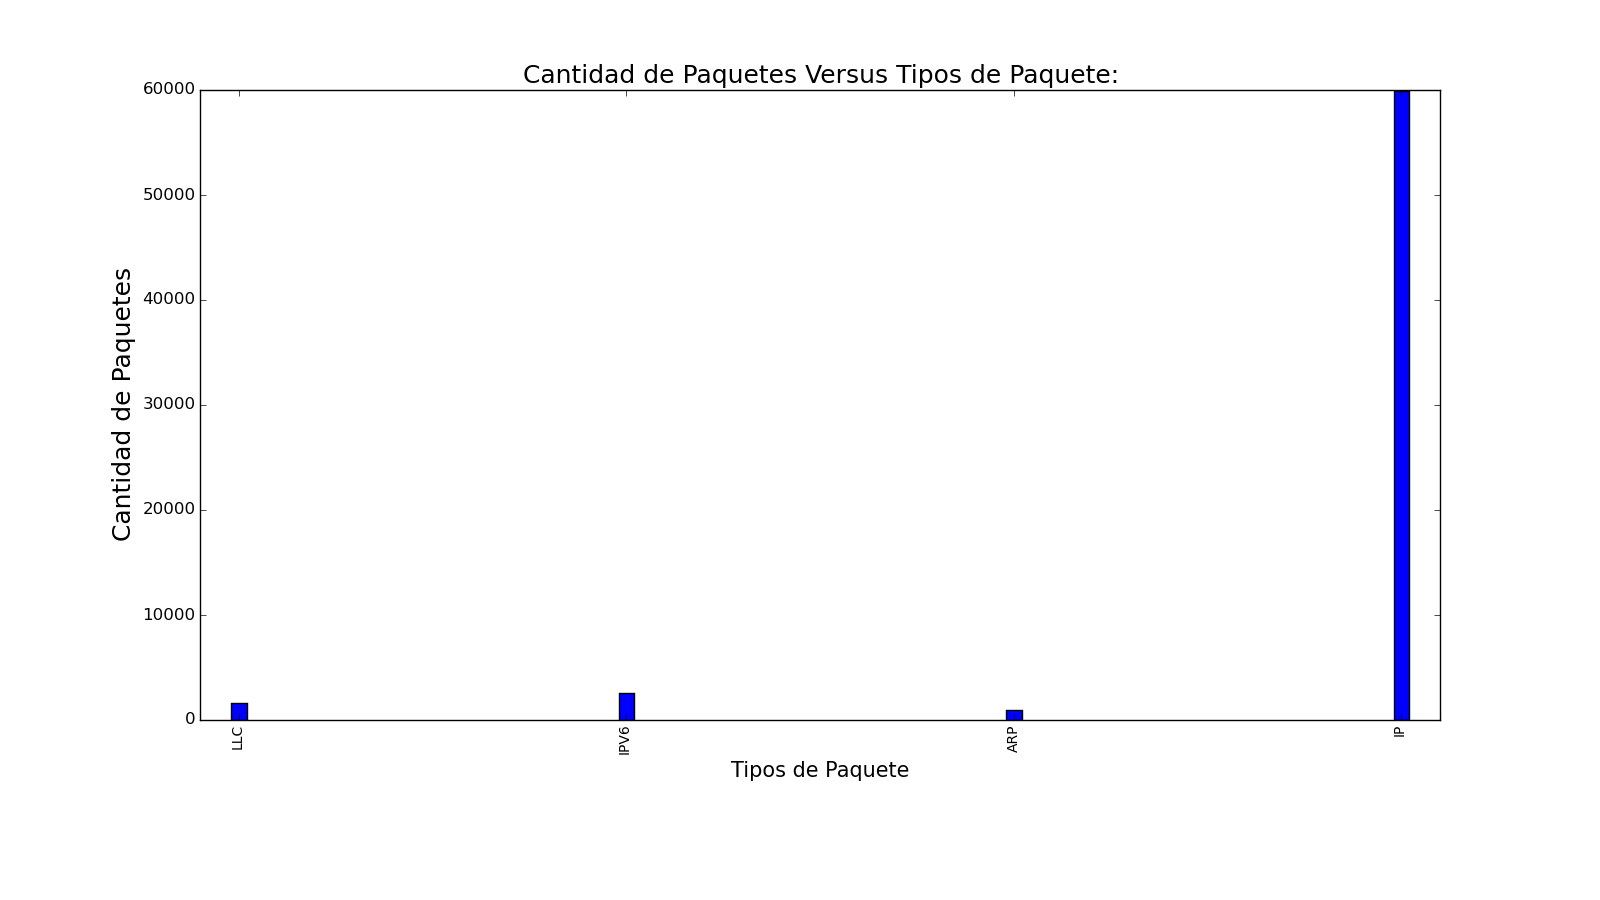
\includegraphics[width=1\textwidth]{../resultados/McDonalds/histogram_types.png}
       \caption{Protocolos de los paquetes capturados}
       \label{red-hogarena-types}
\end{figure}

\begin{figure}[H]
       \centering
       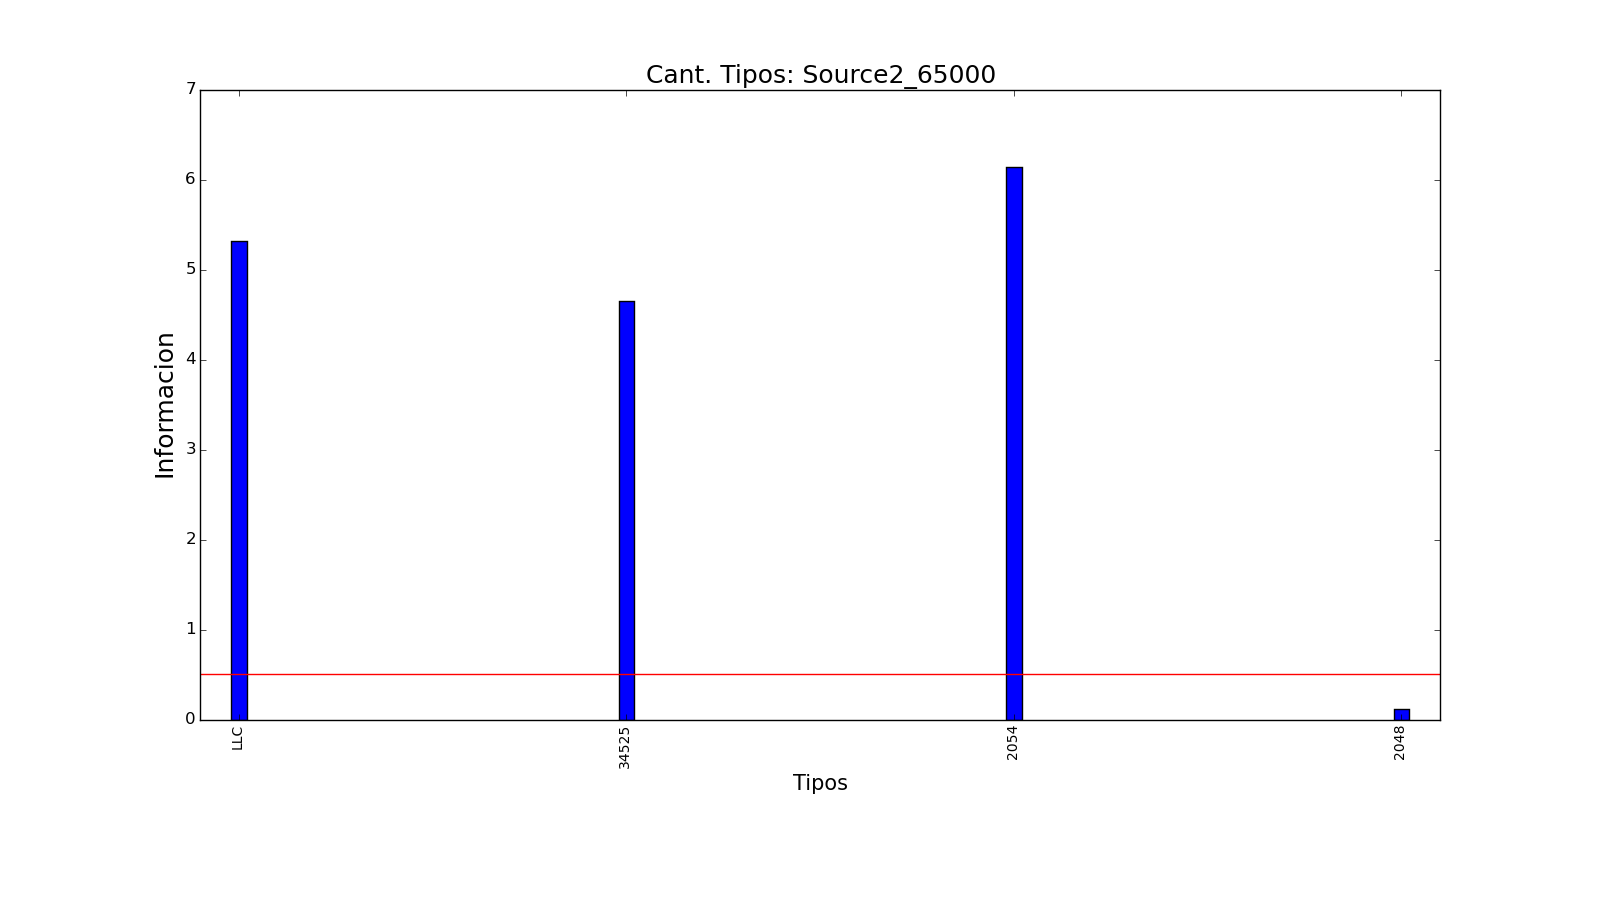
\includegraphics[width=1\textwidth]{../resultados/McDonalds/histogram_types_information.png}
       \caption{Información de los protocolos de los paquetes capturados}
       \label{red-hogarena-types}
\end{figure}


\newpage

\subsection{Red Starbucks}



\newpage

\subsection{Red Laboratorios DC}

Para este experimento, capturamos los paquetes de la LAN Wi-Fi Laboratorios-DC del Departamento de Computació de la FCEyN de la UBA. La medición fue realizada un día Lunes desde las 15hs y durante 15 minutos. La cantidad de paquetes capturados es de 4000. De estos, 164 corresponden al protocolo ARP.

\begin{figure}[H]
       \centering
       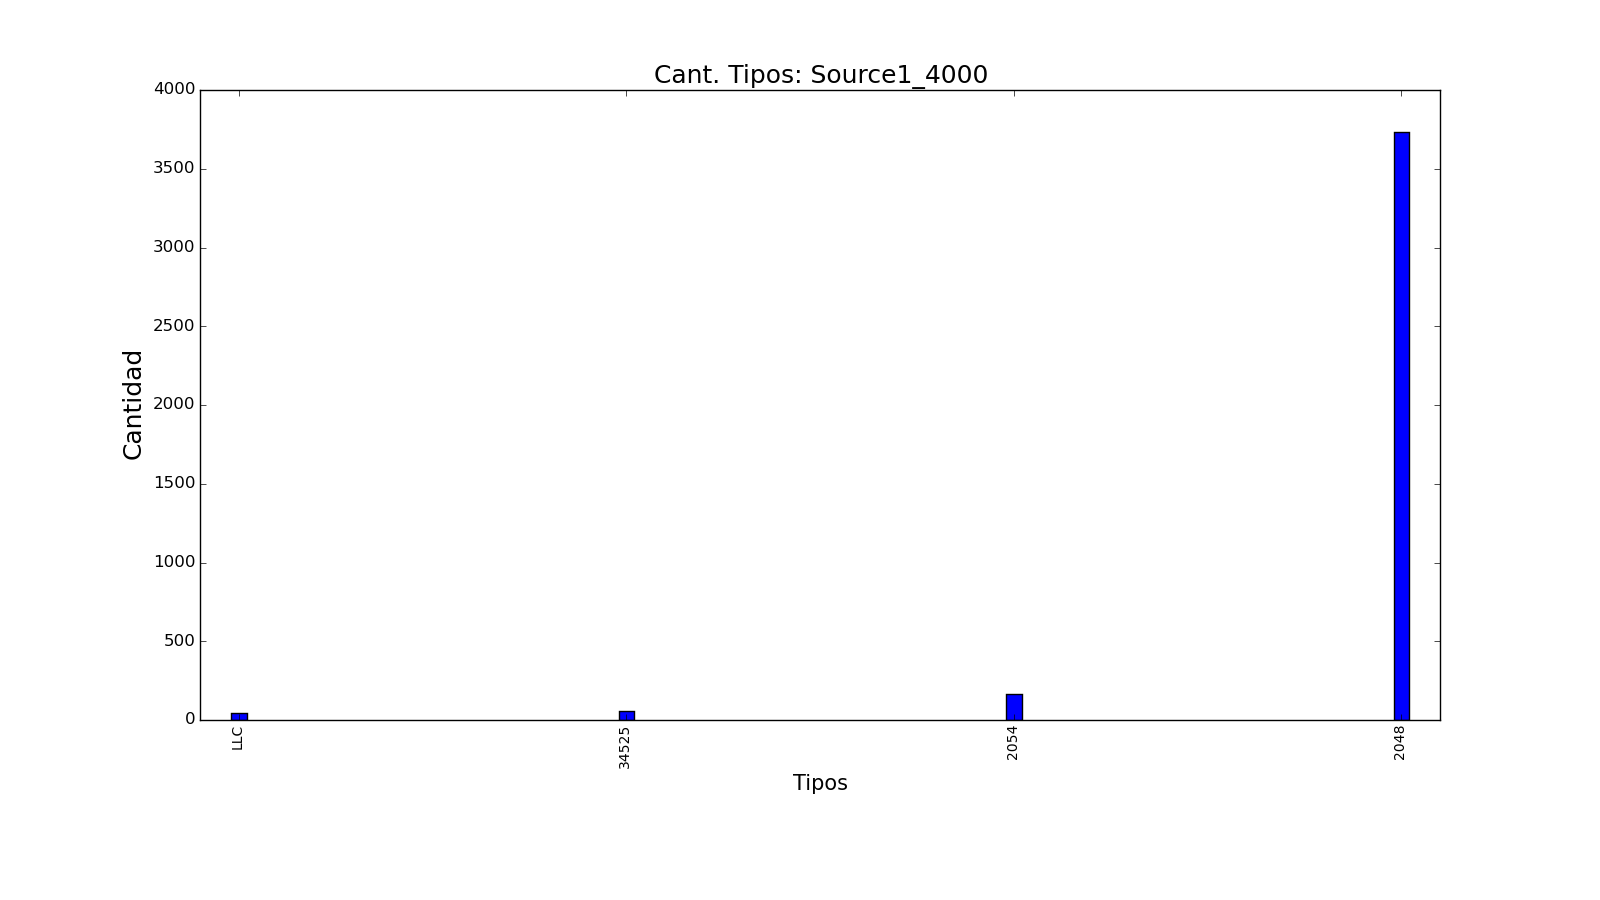
\includegraphics[width=1\textwidth]{../resultados/labo-corrida3/histogram_types.png}
       \caption{Protocolos de los paquetes capturados}
       \label{red-Starbucks-types}
\end{figure}

\begin{figure}[H]
       \centering
       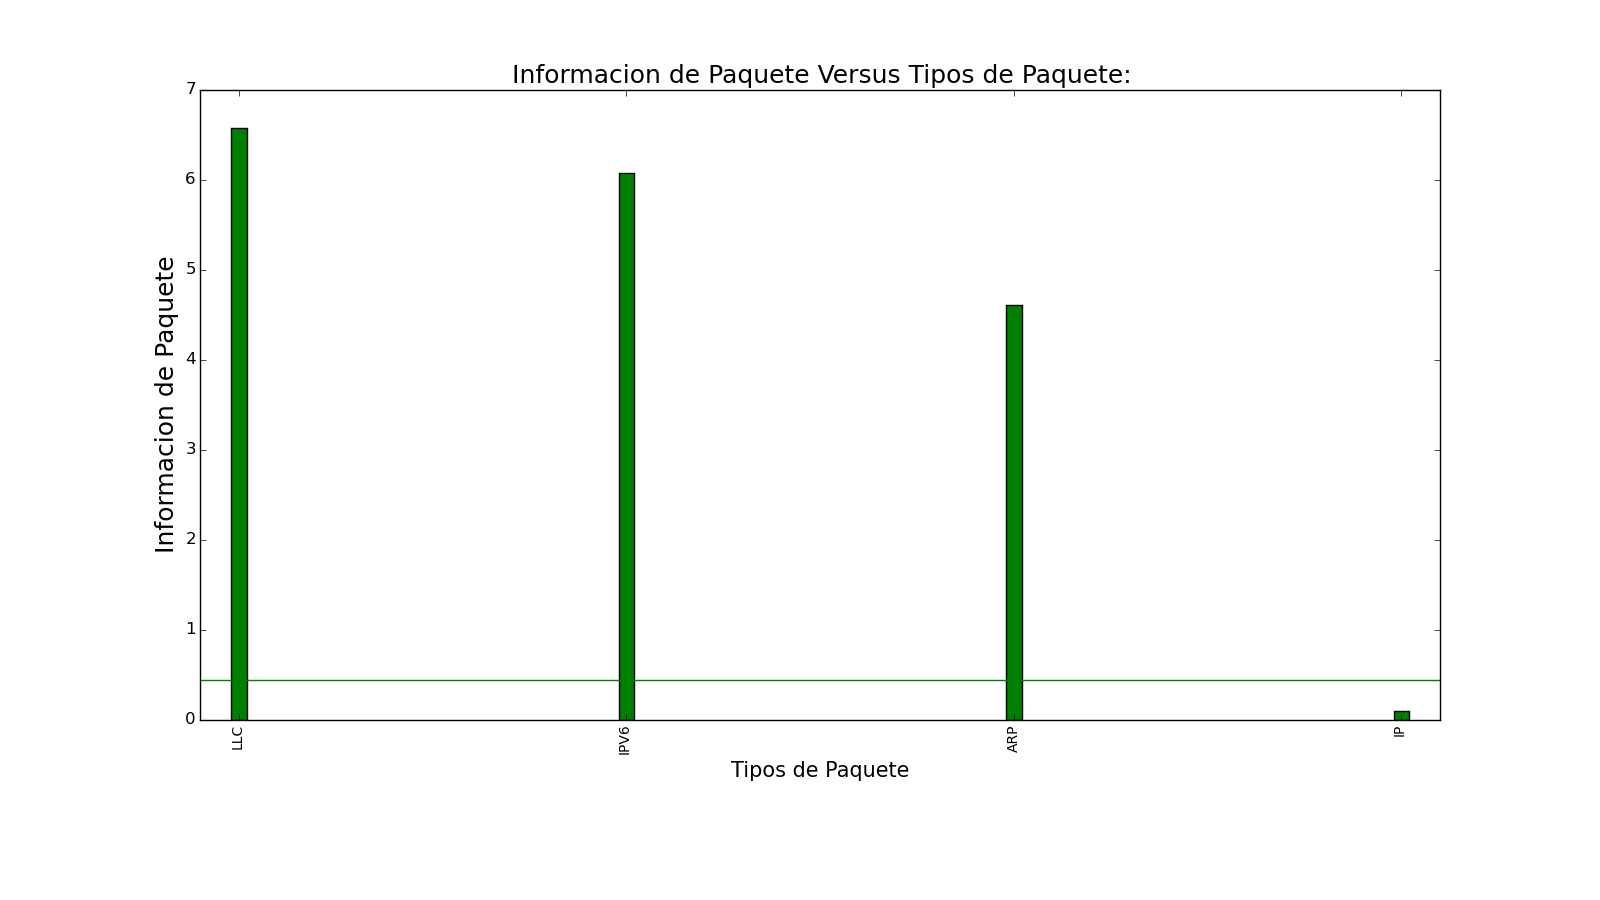
\includegraphics[width=1\textwidth]{../resultados/labo-corrida3/histogram_types_information.png}
       \caption{Información de los protocolos de los paquetes capturados}
       \label{red-Starbucks-types-information}
\end{figure}

Como podemos observar también en este experimento, de acuerdo a nuestra definición de protocolo distinguido, el protocolo IPv4 sería el único distinguido en esta fuente. Es razonable, ya que la cantidad de paquetes IPv4 es mucho mayor que la cantidad de paquetes IPv6, LLC y ARP. La información de los paquetes IPv4 es \textbf{0.0988917569855}, mientras que la entropía de la fuente es \textbf{0.440025436837}. Se observa como la información es claramente menor a la entropía.

\begin{figure}[H]
       \centering
       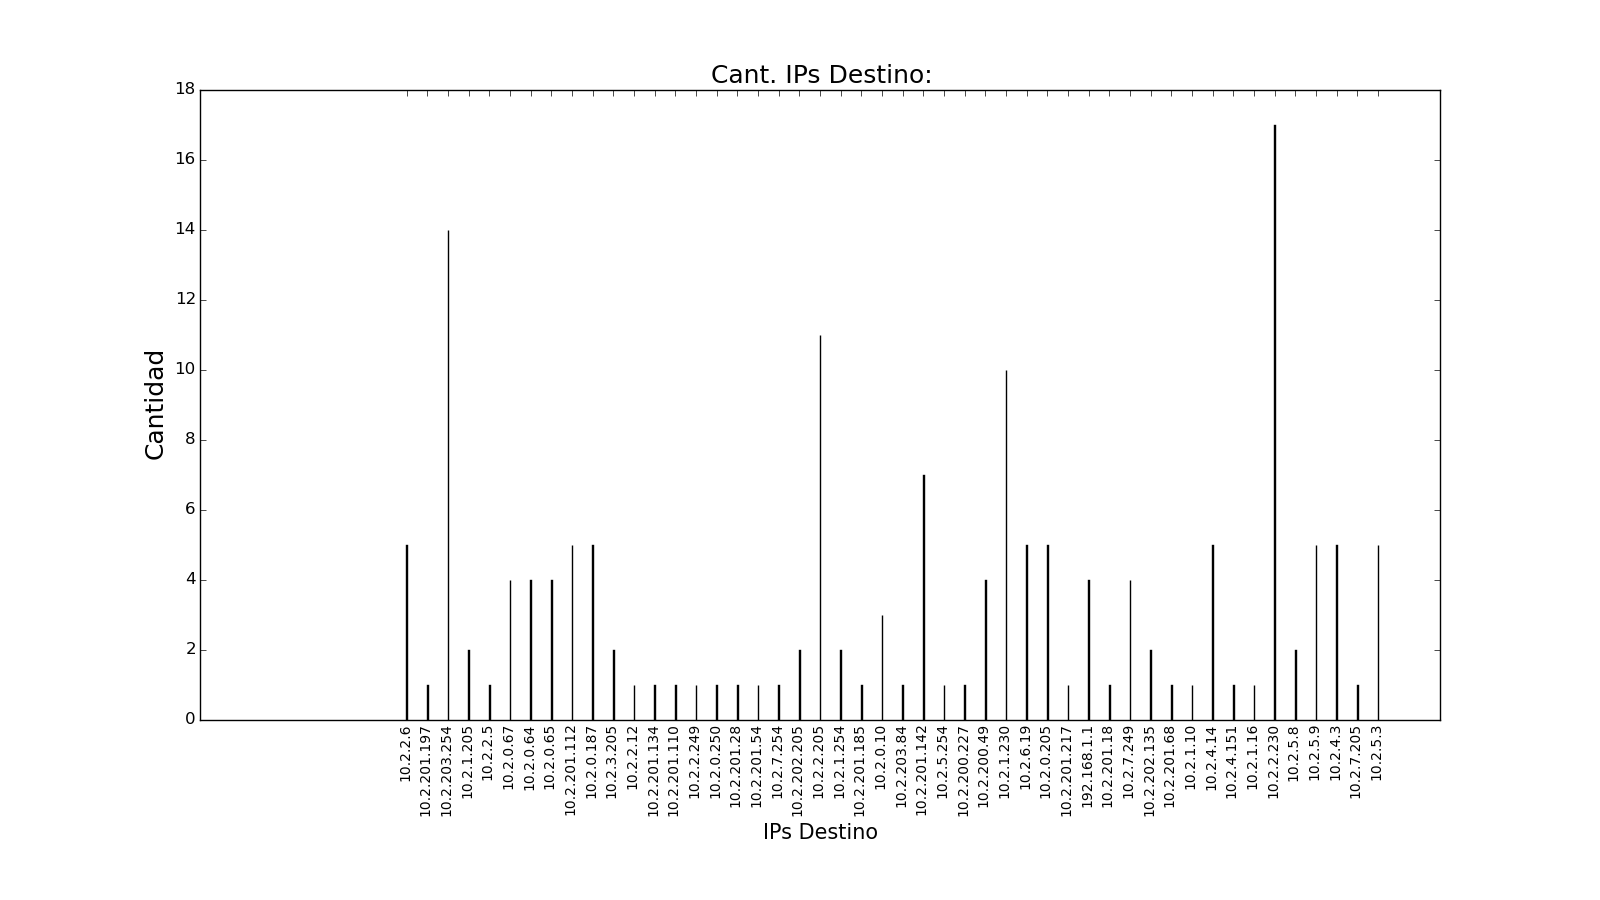
\includegraphics[width=1\textwidth]{../resultados/labo-corrida3/histogram_dst.png}
       \caption{IPs destino de los paquetes ARP}
       \label{red-Starbucks-dst}
\end{figure}

\begin{figure}[H]
       \centering
       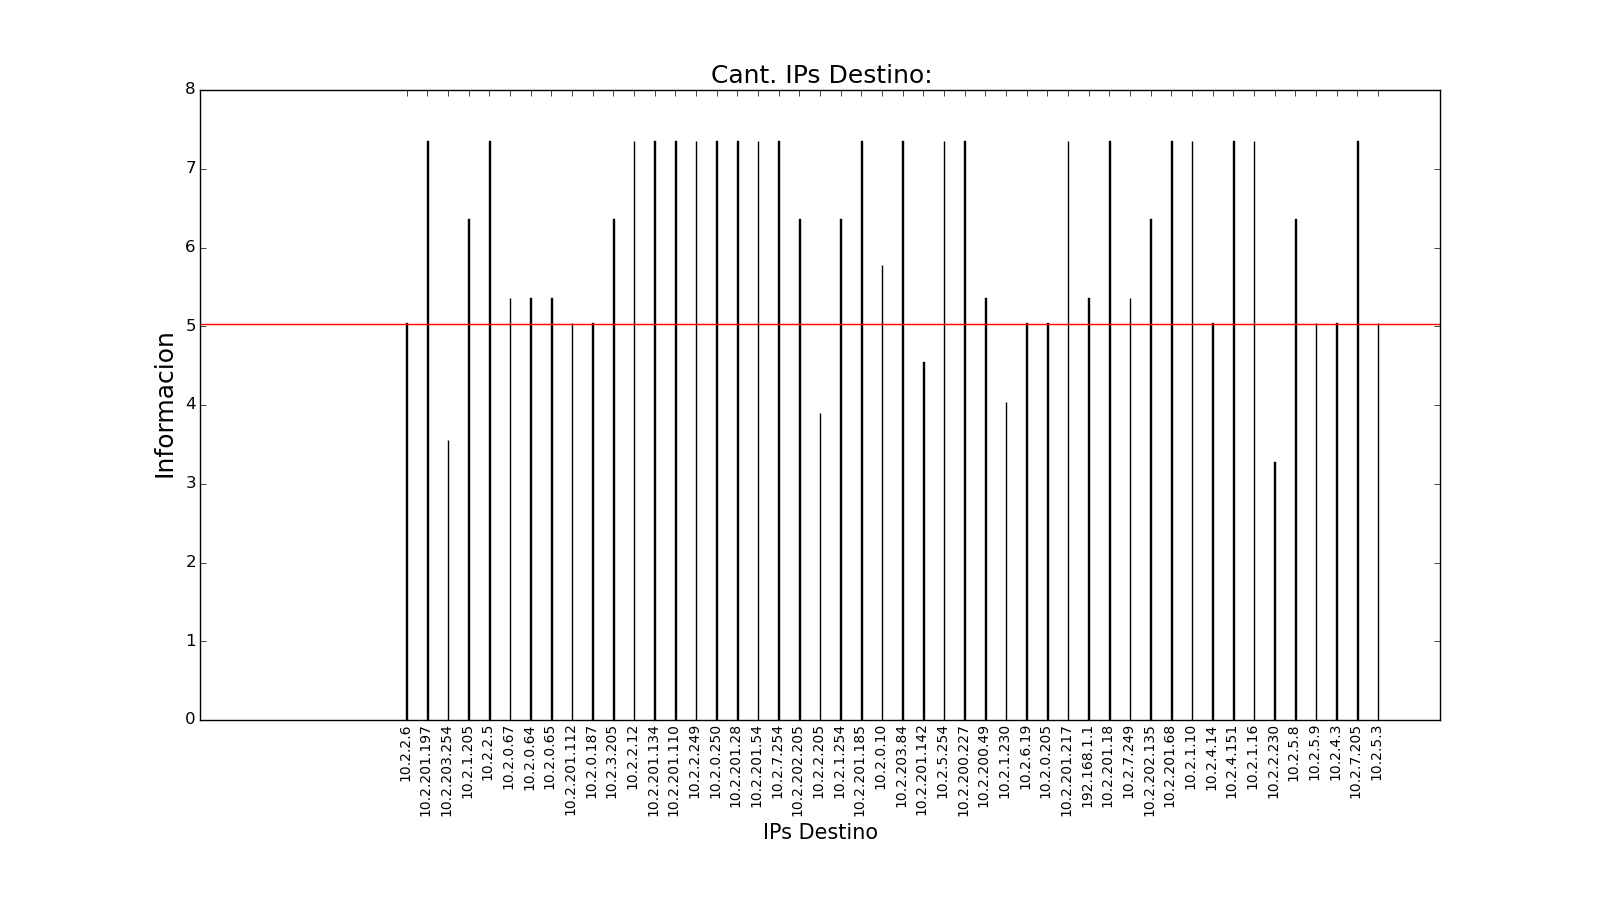
\includegraphics[width=1\textwidth]{../resultados/labo-corrida3/histogram_dst_information.png}
       \caption{Información de IPs destino de los paquetes ARP}
       \label{red-Starbucks-dst-information}
\end{figure}


\begin{figure}[H]
       \centering
       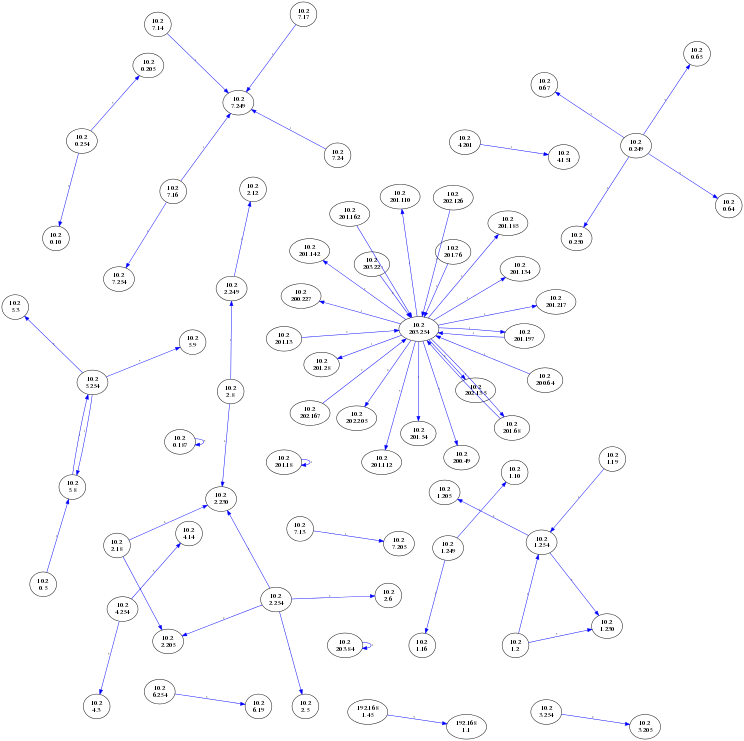
\includegraphics[width=1\textwidth]{../resultados/labo-corrida3/network.png}
       \caption{Tráfico de paquetes ARP}
       \label{red-Starbucks-dst-information}
\end{figure}

Analizando la información de estos gráficos vemos como la IP \textbf{10.2.203.254} parece ser el router: recibe una mayor cantidad de paquetes que casi todas las demás IPs, es un nodo distinguido por ser su información menor a la entropía, y las conexiones que tiene son a las IPs 10.2.200.X, 10.2.201.X y 10.2.202.X, que deben ser subnets.\\

También vemos por ejemplo que la IP \textbf{10.2.2.230} recibe incluso una mayor cantidad de paquetes y  también es un nodo distinguido, pero esa mayor cantidad de paquetes viene desde pocos nodos. Creemos por esto que puede tratarse de algún servidor (de datos, de imágenes, etcétera).

\newpage

\subsection{Red Subte D}

Para el último experimento, capturamos los paquetes de la LAN Wi-Fi Subte-BA de la estación Plaza Italia de la Línea D del Subte de Buenos Aires.La medición fue realizada un día Domingo a las 16.30hs y durante solamente 1 minuto (por motivos externos). Capturamos 1.000 paquetes de los cuales 25 son ARP.

\begin{figure}[H]
       \centering
       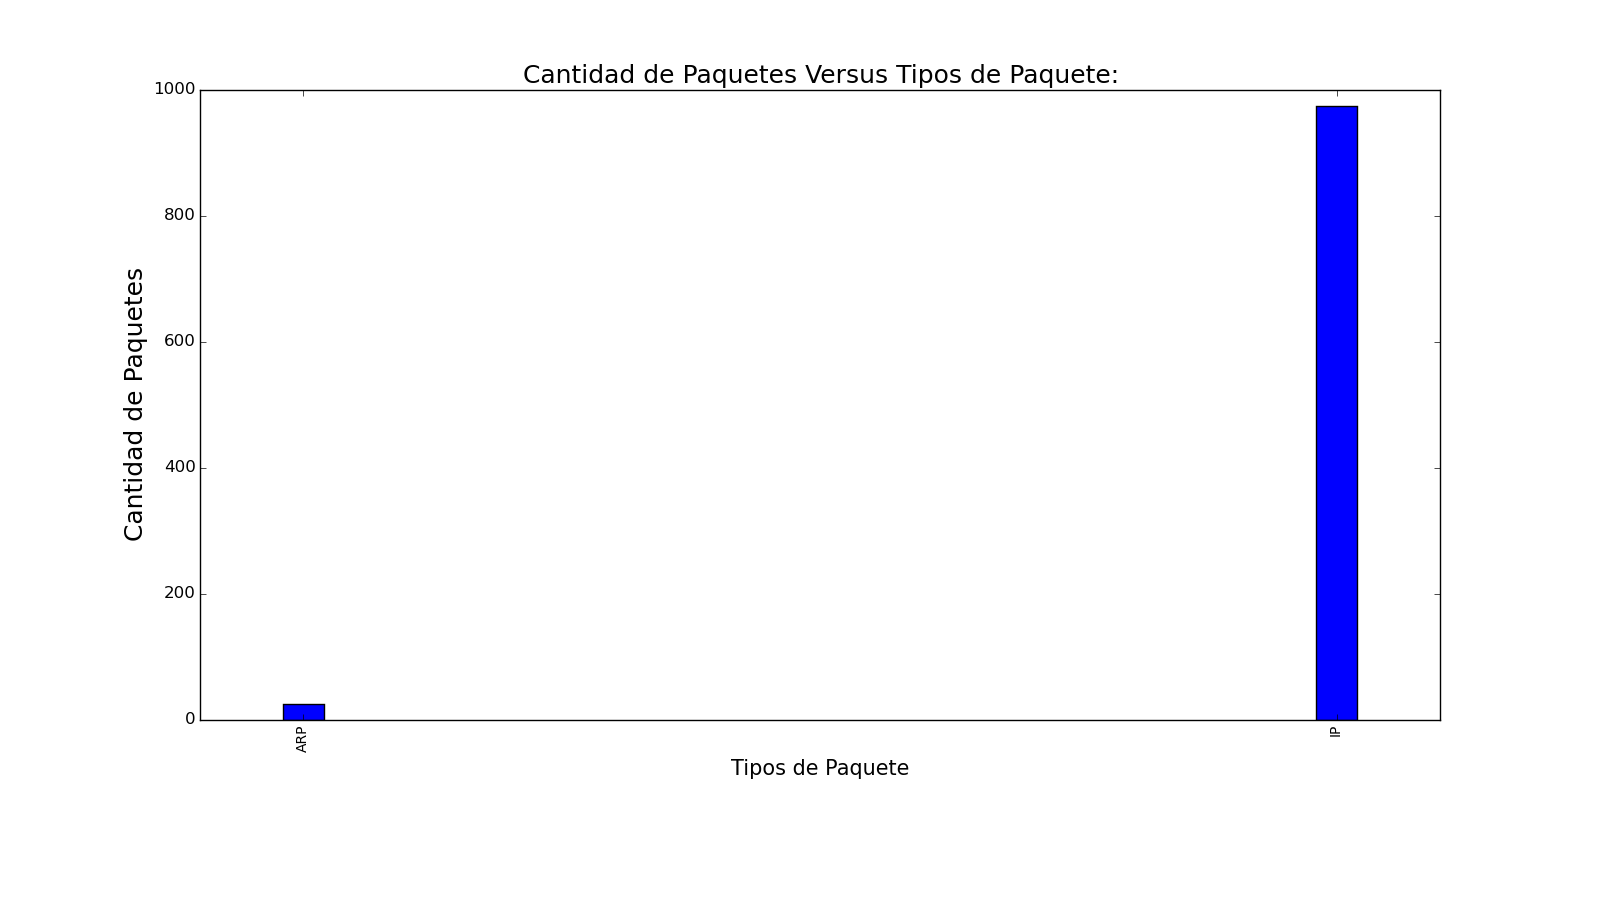
\includegraphics[width=1\textwidth]{../resultados/subte/histogram_types.png}
       \caption{Protocolos de los paquetes capturados}
       \label{red-Starbucks-types}
\end{figure}

En este caso el overhead impuesto por los paquetes ARP es de 2.5\%

\begin{figure}[H]
       \centering
       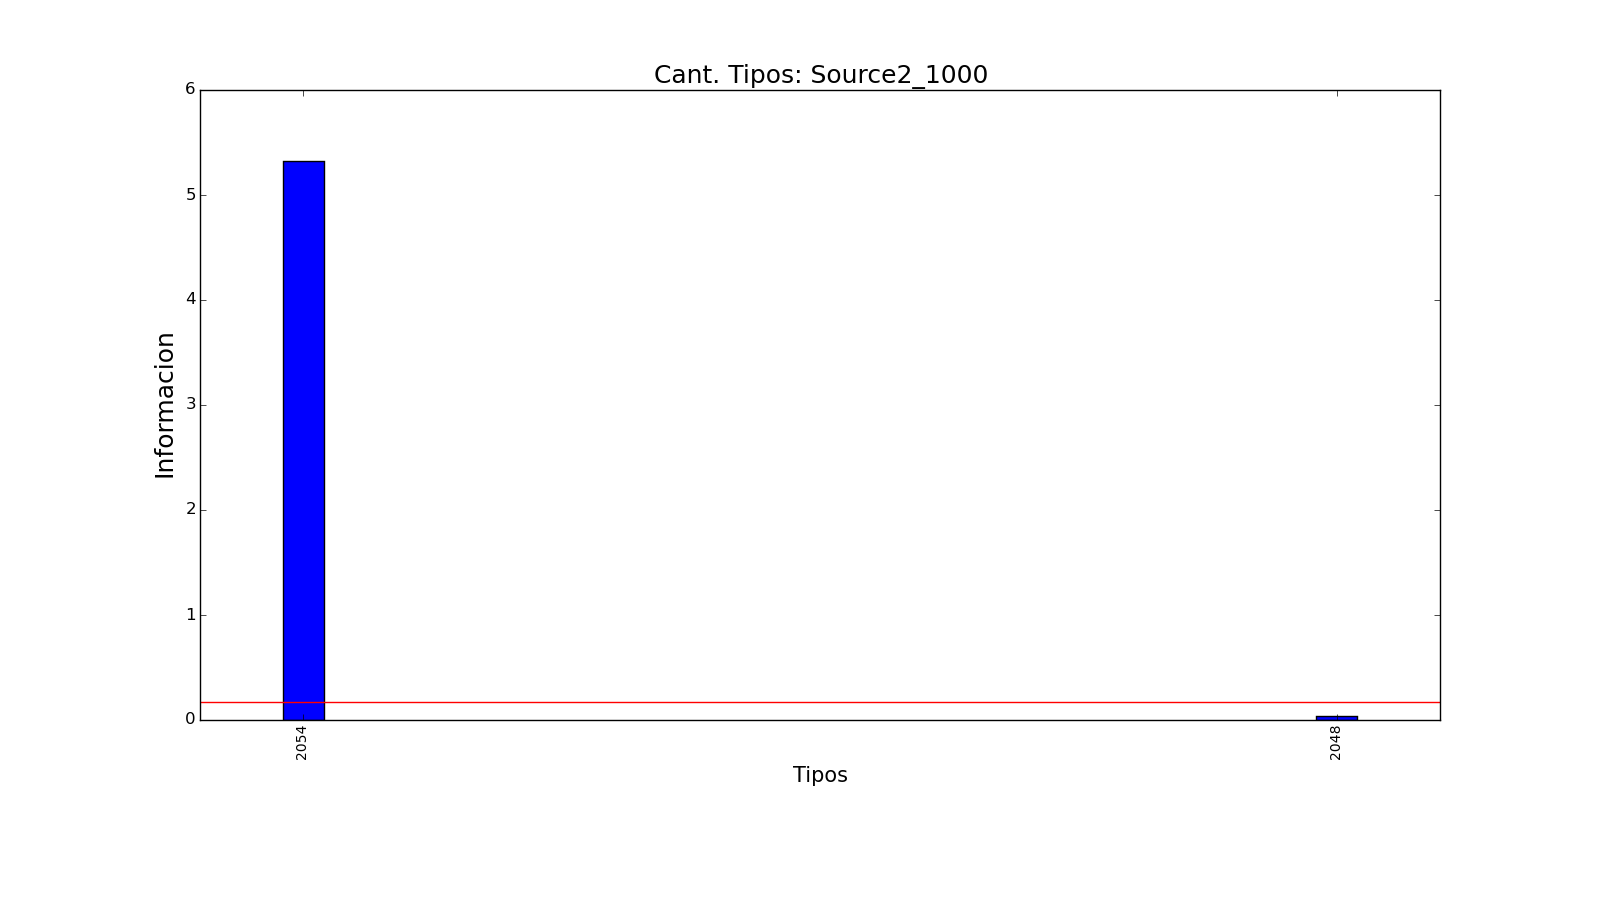
\includegraphics[width=1\textwidth]{../resultados/subte/histogram_types_information.png}
       \caption{Información de los protocolos de los paquetes capturados}
       \label{red-Starbucks-types-information}
\end{figure}

Como podemos también en este experimento, el protocolo IPv4 sería el único distinguido en esta fuente. Es razonable, ya que la cantidad de paquetes IPv4 es mucho mayor que la cantidad de paquetes ARP. La información de los paquetes IPv4 es \textbf{5.32192809489}, mientras que la entropía de la fuente es \textbf{0.168660931497}. Se observa como la información es muy menor a la entropía.

\begin{figure}[H]
       \centering
       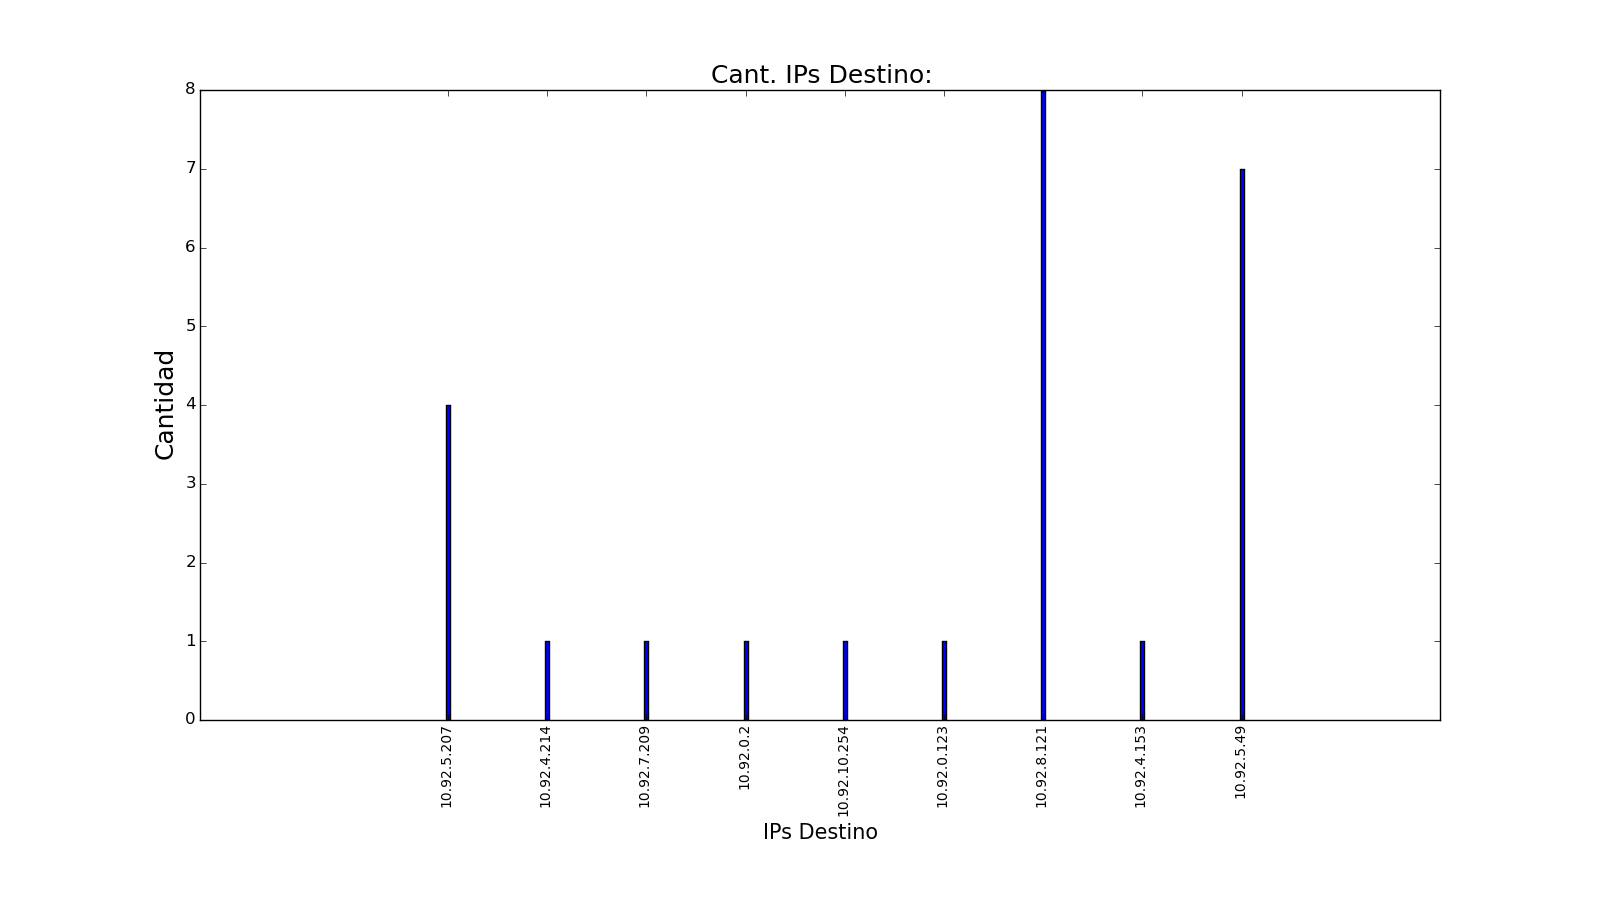
\includegraphics[width=1\textwidth]{../resultados/subte/histogram_dst.png}
       \caption{IPs destino de los paquetes ARP}
       \label{red-Starbucks-dst}
\end{figure}

\begin{figure}[H]
       \centering
       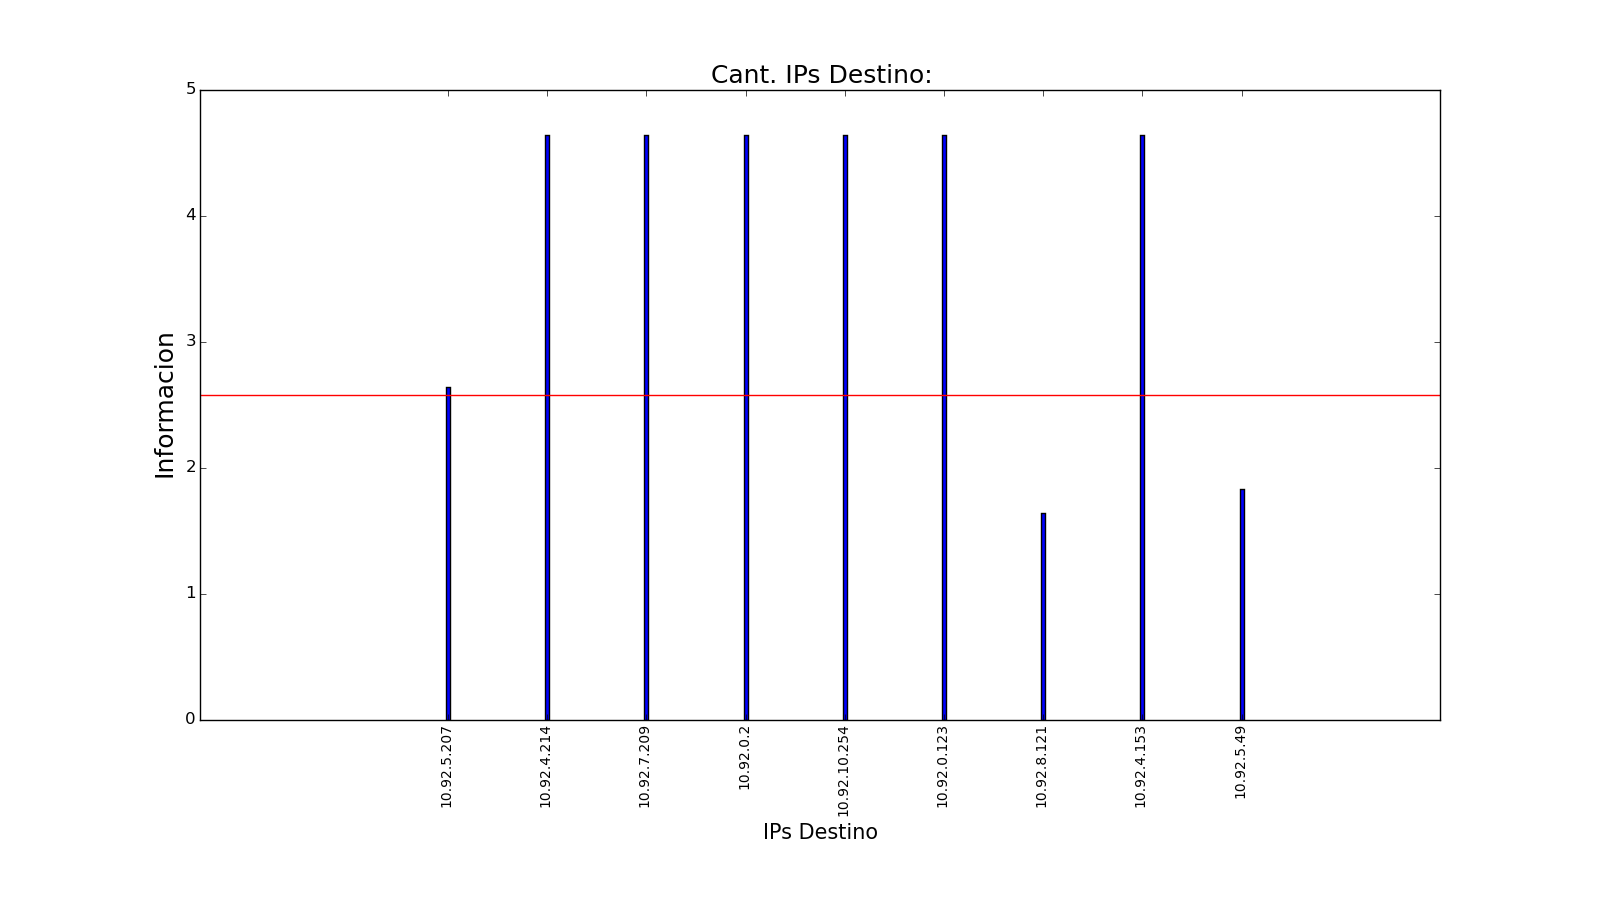
\includegraphics[width=1\textwidth]{../resultados/subte/histogram_dst_information.png}
       \caption{Información de IPs destino de los paquetes ARP}
       \label{red-Starbucks-dst-information}
\end{figure}

\begin{figure}[H]
       \centering
       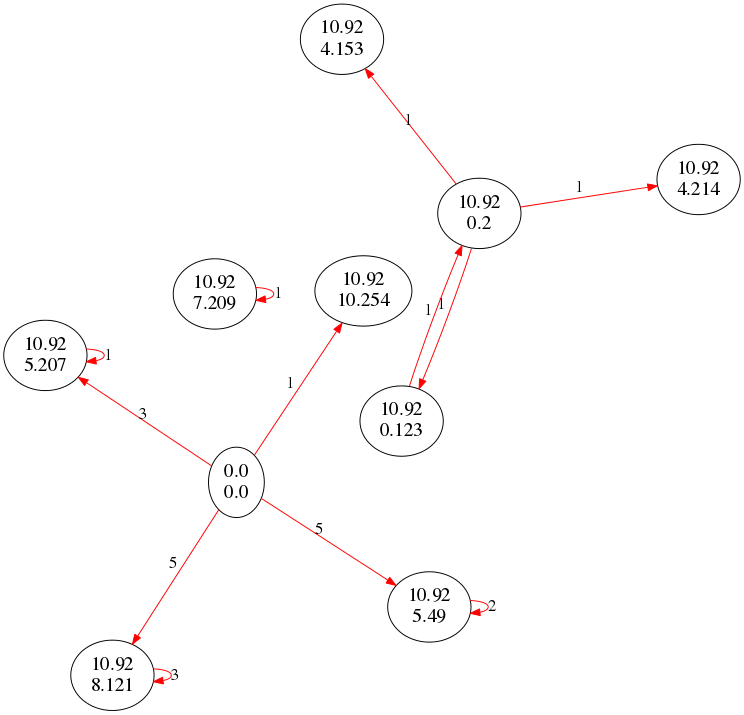
\includegraphics[width=1\textwidth]{../resultados/subte/network.png}
       \caption{Tráfico de paquetes ARP}
       \label{red-Starbucks-dst-information}
\end{figure}

Analizando los gráficos podemos ver que las IPs \textbf{10.92.8.121} y \textbf{10.92.5.49} reciben una mayor cantidad de paquetes que las demás y son nodos distinguidos por ser su información menor a la entropía. Pero los paquetes que reciben tienen como origen a la IP \textbf{0.0.0.0}, que como discutimos en la siguiente sección, son ARP requests que se mandan debido a la ejecución de un protocolo DHCP. No podemos sacar más conclusiones de estos gráficos debido al corto tiempo de intercepción de paquetes.\\
\newpage


